
\input{"C:/Users/spileggi/Google Drive/STAT 330/Lectures/SlideStyle.tex"}



\title[Lecture 1]{SAS Libraries, PROC FREQ, PROC UNIVARIATE}
\author[Pileggi]{Shannon Pileggi}

\institute[STAT 330]{STAT 330}

\date{}


\begin{document}

\begin{frame}
\titlepage
\end{frame}

\begin{frame}
\frametitle{OUTLINE\qquad\qquad\qquad} \tableofcontents[hideallsubsections]
\end{frame}


%===========================================================================================================================
\section[SAS libraries]{SAS libraries}
%===========================================================================================================================

\subsection{}

\begin{frame}
\tableofcontents[currentsection, hideallsubsections]
\end{frame}

\begin{frame}
\ft{Libraries: temporary vs permanent}
SAS stores data sets in a \emph{SAS Library}.  Libraries can be:
\vskip10pt
\ttb{Temporary}
\bi
\item Stored in the \ttt{WORK} folder
\item SAS data sets are deleted when the SAS session closes
\item[]
\ei
\ttb{Permanent}
\bi
\item Some come with SAS, like \ttt{SASHELP}
\item We can also create our own permanent libraries
\item Allows us to create permanent SAS data sets that remain on your computer even after the SAS session closes
\ei
\end{frame}

\begin{frame}
\ft{SAS data set names}
\bi
\item SAS data sets have two-level names: \fbox{\ttt{SASHELP.BASEBALL}}
	\begin{enumerate}
	\item the library reference (\ttt{SASHELP})
	\item the data set name (\ttt{BASEBALL})
	\end{enumerate}
	\item The 2 levels are separated by a period
    \item Capitalization does not matter - these two level names work equivalently: \ttt{SASHELP.baseball}, \ttt{sashelp.BASEBALL}, \ttt{Sashelp.Baseball}
    %\item If the library reference is missing/blank, then it defaults to \ttt{Work}
    \item This naming convention is used in both \ttt{DATA} steps and \ttt{PROCS}
    \item More generally, the naming convention is \fbox{\ttt{LibRef.DataSetName}}
\ei
\end{frame}


\begin{frame}[fragile]
\ft{SAS data set names, another example}
\bmp{0.90\textwidth}
\footnotesize
\hspace*{-1in}
\begin{code}{.0}
PROC IMPORT OUT = \textcolor{OrangeRed}{WORK.babies}
   DATAFILE = "X:/spileggi/Data Sets/babies.csv"
   DBMS = CSV REPLACE;
RUN;

PROC IMPORT OUT = \textcolor{OrangeRed}{babies}
   DATAFILE = "X:/spileggi/Data Sets/babies.csv"
   DBMS = CSV REPLACE;
RUN;
\end{code}
\emp
\vskip10pt
These two code chunks are \textbf{equivalent}. If the library reference is missing/blank, then it defaults to \ttt{WORK}. For both, \\
\begin{itemize}
\item the library reference is \ttt{WORK}
\item the data set name is \ttt{babies}
\end{itemize}
\end{frame}

\begin{frame}
\fto
\begin{clicker}{For each of the following data set names, indicate if we are referring to a (1) temporary SAS data set or (2) a permanent SAS data set.}
\begin{enumerate}
\item \ttt{baseball}
\item \ttt{mylib.baseball}
\item \ttt{work.baseball}
\item \ttt{x.baseball}
\item \ttt{temp.baseball}
\end{enumerate}
\end{clicker}
\end{frame}

\begin{frame}
\ft{Library reference}

\fbox{\ttt{libname LibRef "Computer Address/Location";}}
\bi
\item We can use our own \emph{library reference} to access and save permanent SAS data.  The \ttt{LibRef}
\bi
    \item is limited to 8 characters
    \item must begin with a character
    \item can only contain characters/numbers/underscores
\ei
\item You can think of this as a shortcut to a location on your computer
\item You can see your SAS libraries in the \emph{Explorer window of SAS}
\item If you are navigating in your \emph{computer's} explorer, you will \ttb{not} see the library reference name - just the data set name and extension (\ttt{.sas7bdat})
\ei
\end{frame}

\begin{frame}
\ft{Try it!}
\oyo
\begin{enumerate}
    \item Copy the data set \ttt{adni.sas7bdat} to your flash drive or desktop
    \item Create a library reference called \ttt{flash} for the location of the data set on your flash drive
    \item[] \fbox{\ttt{LIBNAME flash "Computer Address/Location";}}
    \item[] \emph{Remember: You can explore to the data set in your computer and right click on it to identify the location.}
    \item View the contents of the data set
    \item[] \fbox{\ttt{PROC CONTENTS DATA=flash.adni; RUN;}}
\end{enumerate}
\end{frame}

\begin{frame}[fragile]
\ft{Your first DATA step}
In a SAS \texttt{DATA} step we can \emph{create} or \emph{manipulate} data.
\vskip10pt
\bmp{0.75\textwidth}
\footnotesize
\begin{code}{.0}
DATA work.adni_temp ;
RUN;

PROC CONTENTS DATA = work.adni_temp ;
RUN;

PROC PRINT DATA = work.adni_temp ;
RUN;
\end{code}
\emp
\vskip10pt
Here, we are creating a \emph{brand new}, temporary data set called \ttt{adni\_temp} in the work library.\\
\vskip10pt
\oyo How many observations and variables are in the \ttt{work.adni\_temp} data set?
\end{frame}

\begin{frame}[fragile]
\ft{Using the SET statement, demo 1}
The \ttt{SET} statement allows you to make a copy of an existing data set, as well as perform calculations/manipulations on the data.
\vskip5pt
\bmp{0.75\textwidth}
\footnotesize
\begin{code}{.0}
DATA work.adni_temp ;
    SET flash.adni;
RUN;

PROC CONTENTS DATA = work.adni_temp ;
RUN;
\end{code}
\emp
\vskip10pt
Here, we are creating a \emph{brand new}, temporary data set called \ttt{adni\_temp} in the work library.  This data set contains a copy of the permanent \ttt{adni} data set located in the \ttt{flash} library.  \\
\vskip10pt
\oyo How many observations and variables are in the \ttt{work.adni\_temp} data set?
\end{frame}

\begin{frame}[fragile]
\ft{Using the SET statement, demo 2}
\bmp{0.75\textwidth}
\footnotesize
\begin{code}{.0}
DATA flash.adni2 ;
    SET flash.adni;
RUN;

PROC CONTENTS DATA = flash.adni2 ;
RUN;
\end{code}
\emp
\vskip10pt
Here, we are creating a \emph{brand new}, permanent SAS data set called \ttt{adni2} in the flash library.  This data set contains a copy of the permanent \ttt{adni} data set located in the \ttt{flash} library.  \\
\vskip10pt
\oyo How many observations and variables are in the \ttt{flash.adni2} data set?  Examine your desktop / flash drive to verify that this data set was created.
\end{frame}

%\begin{frame}
%\ft{Using the SET statement}
%The \ttt{SET} statement allows you to make a copy of an existing data set, as well as perform calculations/manipulations on the data.
%\bi
%\item[]
%\item[Demo 1] \fbox{\ttt{data oscars\textunderscore temp; set flash.oscars; run;}}
%\item[] Creates a \emph{temporary} SAS data set named \ttt{oscars\textunderscore temp} which contains the \ttt{flash.oscars} data.
%\item[]
%\item[Demo 2] \fbox{\ttt{data flash.oscars2; set flash.oscars; run;}}
%\item[] Creates a \emph{permanent} SAS data set named \ttt{oscars2}, in the same location as \ttt{oscars}, which contains the \ttt{flash.oscars} data.
%\ei
%\end{frame}

\begin{frame}
\ft{Discussion}
\begin{clicker}{Suppose I want to create a permanent data set named \ttt{cookie} that is stored in the SAS library \ttt{monster}. Which \ttt{libname} statement is correct?}
\begin{enumerate}
\item \ttt{libname cookie.monster "Computer Location";}
\item \ttt{libname cookie "Computer Location";}
\item \ttt{libname monster "Computer Location";}
\item \ttt{libname cookie monster "Computer Location";}
\item \ttt{libname monster.cookie "Computer Location";}
\end{enumerate}
\end{clicker}
\end{frame}

%===========================================================================================================================
\section[PROC FREQ]{PROC FREQ}
%===========================================================================================================================
\subsection{}
\begin{frame}
\tableofcontents[currentsection, hideallsubsections]
\end{frame}

\begin{frame}[fragile]
\ft{PROC FREQ}
\bmp{0.6\textwidth}
\footnotesize
\begin{code}{.0}
proc freq data=datasetname;
    table var1 var1*var2 / \emph{options};
run;
\end{code}
\emp
\bi
\item Obtains counts of \emph{numeric} and \emph{character} variable values.
\item For two way tables, \ttt{var1} goes on rows and \ttt{var2} goes on columns
\item \ttt{table} options:
	\bi
	\item \ttt{list} - modifies output to list format
	\item \ttt{missing} - includes number of missing in counts
    \item \ttt{nopercent} - suppresses overall percentages
    \item \ttt{nocol} - suppresses column percentages
    \item \ttt{norow} - suppresses row percentages
    \item \ttt{out=} - save frequencies/percents to a data set
	\ei
\ei
\end{frame}

\begin{frame}[fragile]
\ft{Example code}
\bmp{1.0\textwidth}
\footnotesize
\begin{code}{.0}
*all variables in data set;
PROC FREQ DATA = flash.adni; RUN;

*one-way and two-way contingency table;
PROC FREQ DATA = flash.adni;
    TABLES dx dx*gender ;
RUN;

*two-way contingency table converted to list style;
PROC FREQ DATA = flash.adni;
    TABLES dx*gender / LIST MISSING NOPERCENT;
RUN;
\end{code}
\emp
\end{frame}


\begin{frame}[fragile]
\fto
\bmp{1.0\textwidth}
\footnotesize
\begin{code}{.0}
PROC FREQ DATA = flash.adni;
    TABLES dx*gender / \textcolor{OrangeRed}{\emph{options}};
RUN;
\end{code}
\emp
\begin{clicker}{Which options would you use to obtain the percent of males that have a normal diagnosis?}
\begin{enumerate}
\item \ttt{list missing}
\item \ttt{missing nopercent}
\item \ttt{norow nocol}
\item \ttt{nocol nopercent}
\item \ttt{norow nopercent}
\end{enumerate}
\end{clicker}
\end{frame}

\begin{frame}[fragile]
\ft{Chi-square test}
\bmp{0.5\textwidth}
\footnotesize
\begin{code}{.0}
PROC FREQ DATA = flash.adni;
    TABLES dx*gender / \textcolor{OrangeRed}{\emph{CHISQ}};
RUN;
\end{code}
\emp
\bmp{0.05\textwidth} \hspace{1in} \emp
\bmp{0.5\textwidth}
% trim={<left> <lower> <right> <upper>}
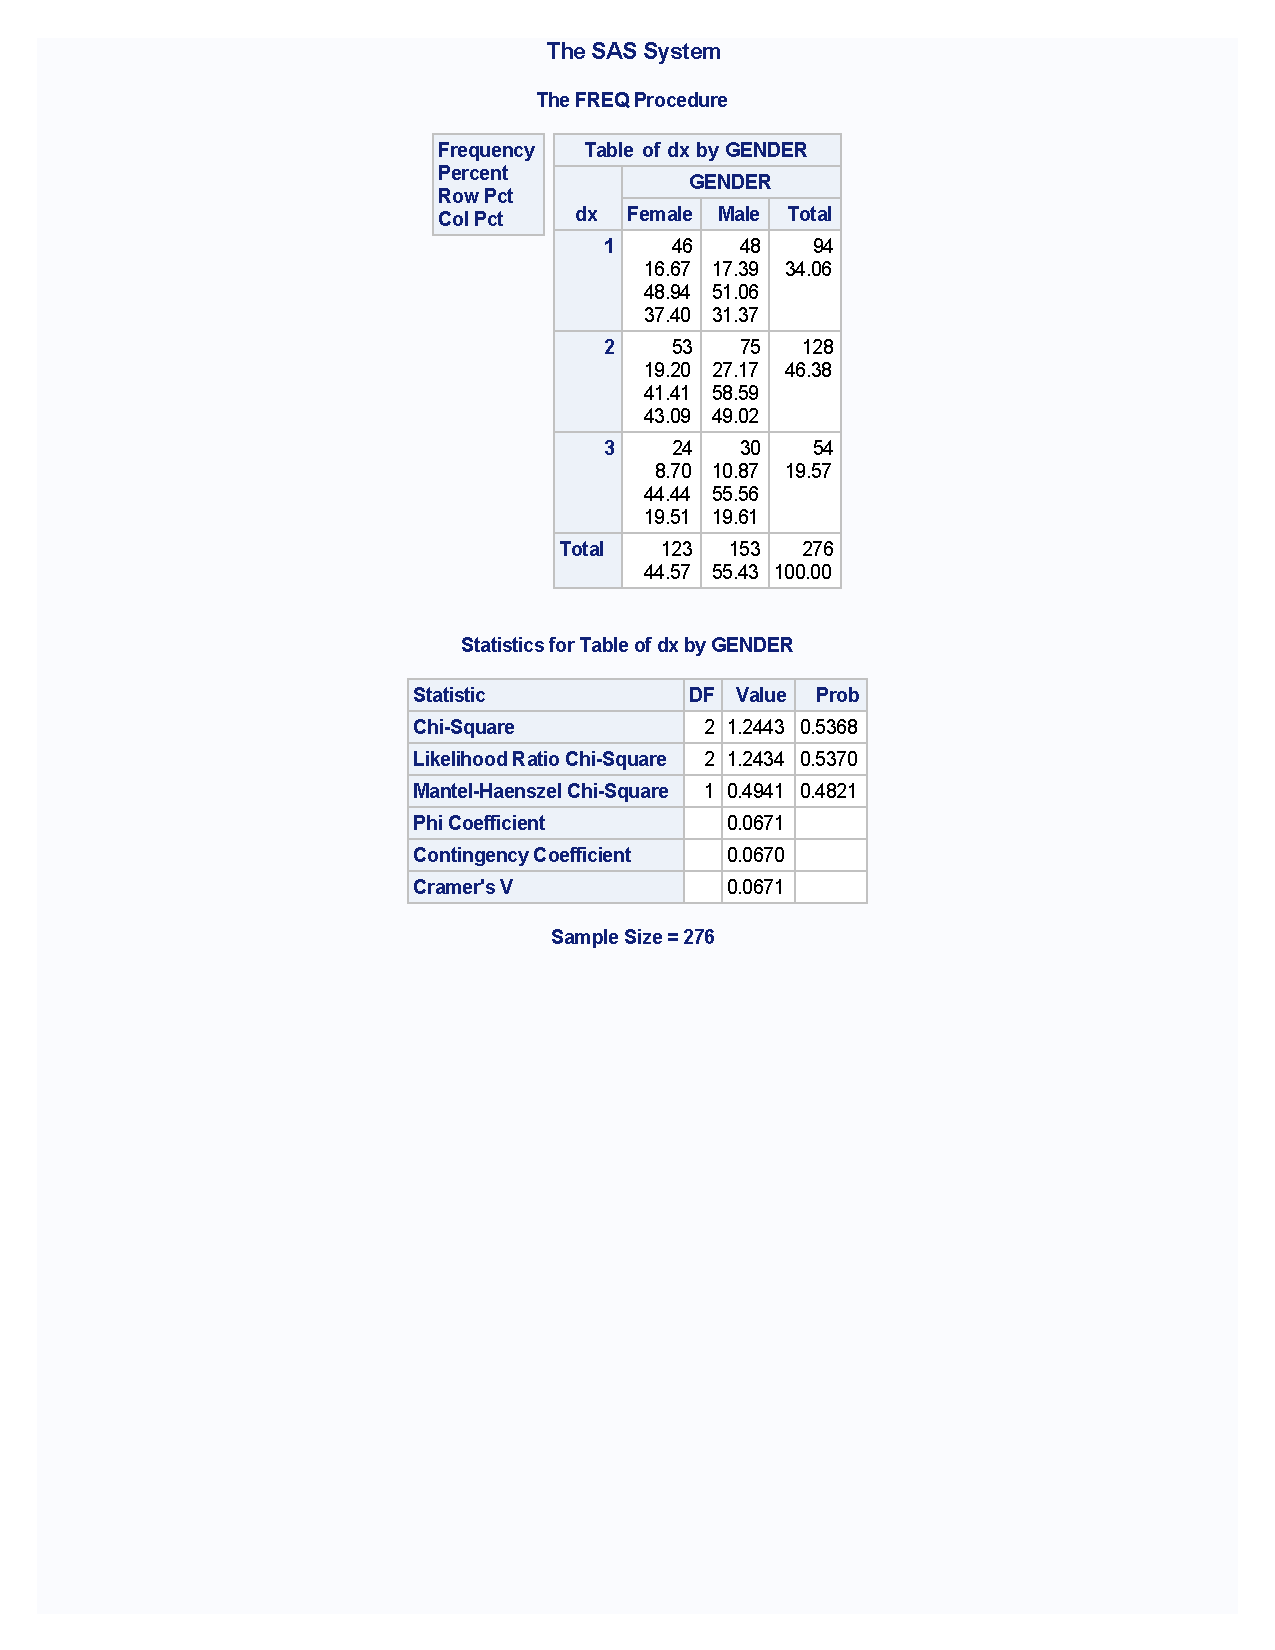
\includegraphics[trim={6cm 12.5cm 6cm 10cm},clip,width=1.0\textwidth]{L3_chisq.pdf}
\emp
\vskip10pt
$H_0$: there is no association between gender and diagnosis \\
$H_a$: there is an association between gender and diagnosis
\vskip10pt
\oyo What is the conclusion?
\end{frame}

%===========================================================================================================================
\section[PROC UNIVARIATE]{PROC UNIVARIATE}
%===========================================================================================================================
\subsection{}
\begin{frame}
\tableofcontents[currentsection, hideallsubsections]
\end{frame}

\begin{frame}[fragile]
\ft{PROC UNIVARIATE}
\bi
\item \ttt{PROC UNIVARIATE} also produces descriptive and some inferential statistics
\item much more detailed output than \ttt{PROC MEANS}
\item default is to produce results for all numeric variables
\item can also produce graphs
\ei
\bmp{1.0\textwidth}
\footnotesize
\begin{code}{.0}
PROC UNIVARIATE DATA = flash.adni ;
RUN;
\end{code}
\emp
\end{frame}

\begin{frame}[fragile]
\ft{One sample t-test}
\bmp{0.5\textwidth}
\footnotesize
\begin{code}{.0}
PROC UNIVARIATE
    DATA = flash.adni
    CIBASIC LOCATION = 70 ;
    VAR age ;
RUN;
\end{code}
\bi
\item \texttt{CIBASIC} computes a confidence interval for the population mean age
\item \texttt{LOCATION} specifies the null hypothesis value
\ei
\emp
\bmp{0.05\textwidth} \hspace{1in} \emp
\bmp{0.5\textwidth}
% trim={<left> <lower> <right> <upper>}
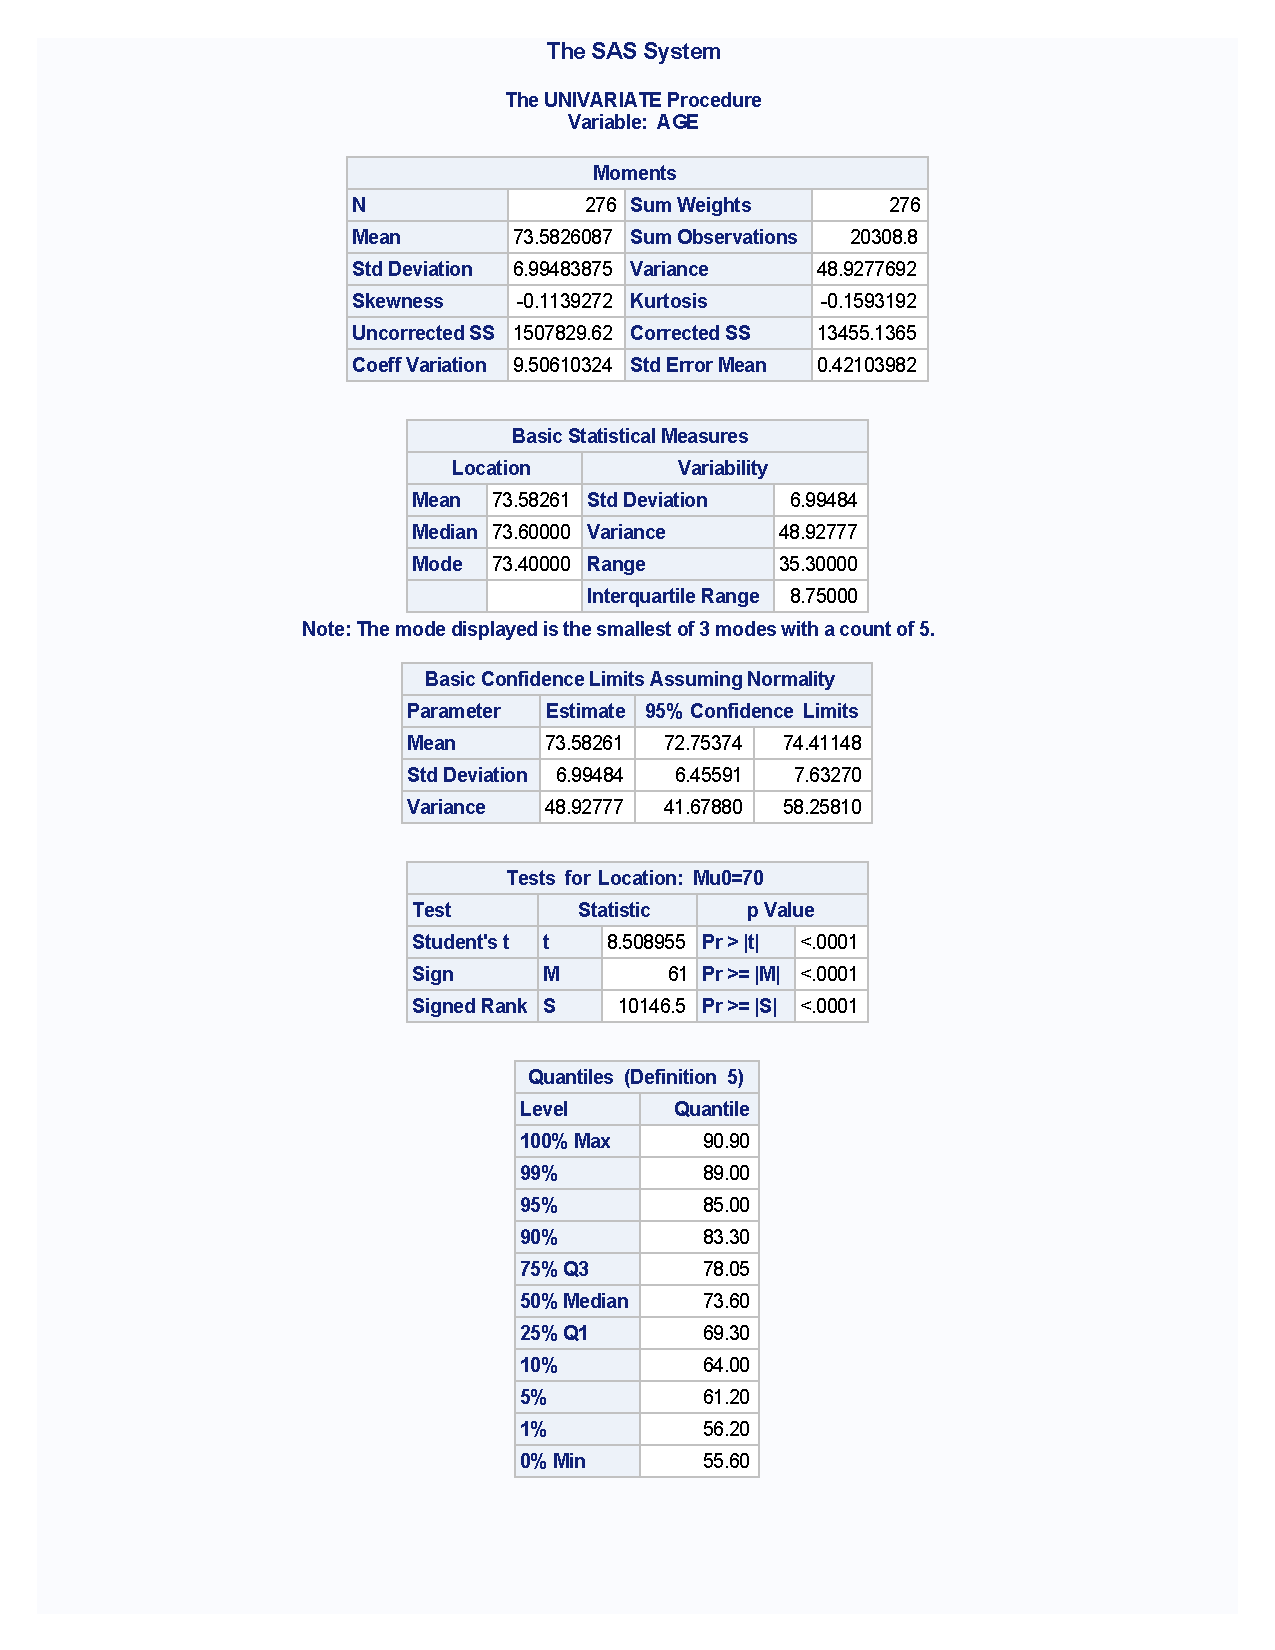
\includegraphics[trim={6cm 10.5cm 6cm 11cm},clip,width=1.0\textwidth]{L3_onesamplet.pdf}\\
\vskip10pt
$H_0$: $\mu=70$ vs $H_a$: $\mu\neq70$\\
\vskip10pt
\oyo What is the interpretation of the result?
\emp

\end{frame}

\begin{frame}[fragile]
\ft{PROC UNIVARIATE}
\bi
\item \ttt{PROC UNIVARIATE} has many more options
\item Like \ttt{PROC UNIVARIATE}, can use \texttt{CLASS} or \texttt{BY} statements
\item Can also produce graphs
\ei
\bmp{0.6\textwidth}
\footnotesize
\begin{code}{.0}
PROC UNIVARIATE DATA = flash.adni ;
   CLASS dx;
   VAR MMSE;
   HISTOGRAM MMSE / NORMAL;
RUN;
\end{code}
\emp
\bmp{0.4\textwidth}
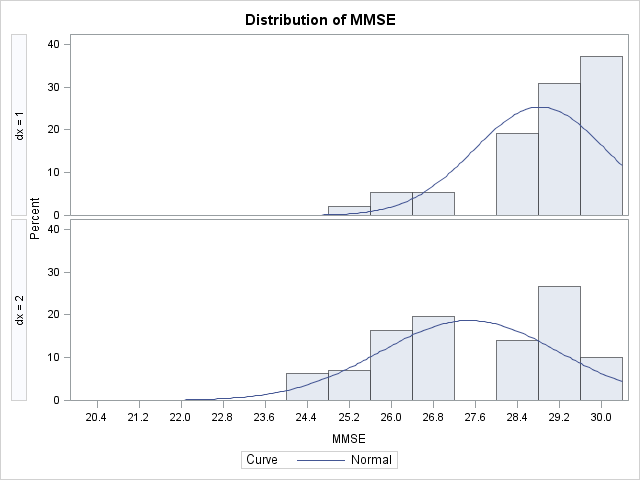
\includegraphics[width=1.0\textwidth]{L3_hist.png}\\
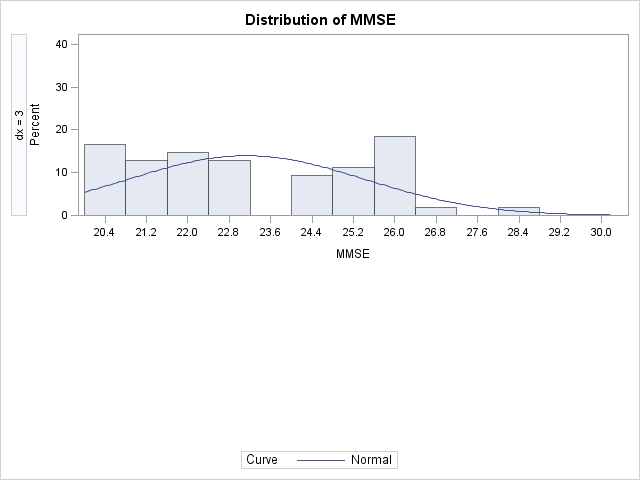
\includegraphics[width=1.0\textwidth]{L3_hist2.png}
\emp
\end{frame}

%===========================================================================================================================
\section[Discussion]{Discussion}
%===========================================================================================================================
\subsection{}
\begin{frame}
\tableofcontents[currentsection, hideallsubsections]
\end{frame}

\begin{frame}
\fto
\begin{tabular}{r|l}
\ttt{APOE4} & Type of APOE4 variant (genetics)  \\
            & \hspace{0.2in} 0 - No copies of the ApoE4 allele\\
            & \hspace{0.2in} 1 - One copy of the ApoE4 allele\\
            & \hspace{0.2in} 2 - Two copies of the ApoE4 allele\\
\end{tabular}
\vskip10pt
\begin{clicker}{Which \ttt{PROC} would you use to \emph{summarize} \ttt{APOE4}?}
\begin{enumerate}
    \item \ttt{PROC PRINT}
    \item \ttt{PROC CONTENTS}
    \item \ttt{PROC MEANS}
    \item \ttt{PROC UNIVARIATE}
    \item \ttt{PROC FREQ}
\end{enumerate}
\end{clicker}
\end{frame}


\begin{frame}
\fto
\begin{tabular}{r|l}
\ttt{ADAS} & Alzheimer's Disease Assessment Scale (larger \\
           & scores indicate greater dysfuction)\\
\end{tabular}
\vskip10pt
\begin{clicker}{Which \ttt{PROC} would you use to see if there are any unusual/outlier/erroneous values of \ttt{ADAS}?}
\begin{enumerate}
    \item \ttt{PROC PRINT}
    \item \ttt{PROC CONTENTS}
    \item \ttt{PROC MEANS}
    \item \ttt{PROC UNIVARIATE}
    \item \ttt{PROC FREQ}
\end{enumerate}
\end{clicker}
\end{frame}

%===========================================================================================================================
\section[ADNI data]{About the ADNI data}
%===========================================================================================================================
\subsection{}
\begin{frame}
\tableofcontents[currentsection, hideallsubsections]
\end{frame}
%\begin{frame}
%\tableofcontents[currentsection, hideallsubsections]
%\end{frame}


\begin{frame}
\ft{The Data}
\bi
\item Alzheimer's Disease (AD) is a serious mental illness that affects an estimated 5.3 million Americans; it is the most common cause of dementia among the elderly.
\item Characterized by a progressive cognitive decline, AD has been notoriously difficult to diagnose due to symptom-overlap with other mental disorders; until recently, AD could only be confirmed posthumously.
\item The Alzheimer's Disease Neuroimaging Initiative (ADNI) is a longitudinal study that began in 2005, and is designed to track AD biomarkers, identify at-risk patients, and evaluate the efficacy of novel treatments.
\item The study consists of healthy individuals (the control group) as well as adults with early Alzheimer's Disease (AD). \url{http://adni.loni.usc.edu/about/}.
\ei
\end{frame}

\begin{frame}
\ft{The Variables}
\begin{tabular}{r|l}
\ttt{DX}   &  Alzheimer's disease diagnosis\\
           & \hspace{0.2in} 1 - Normal cognitive function\\
           & \hspace{0.2in} 2 - Mild cognitive impairment\\
           & \hspace{0.2in} 3 - Alzheimer's disease \\
\ttt{AGE} &  Age (years) \\
\ttt{APOE4} & Type of APOE4 variant (genetics)  \\
            & \hspace{0.2in} 0 - No copies of the ApoE4 allele\\
            & \hspace{0.2in} 1 - One copy of the ApoE4 allele\\
            & \hspace{0.2in} 2 - Two copies of the ApoE4 allele\\
\ttt{GENDER} &  Patient gender  \\
\ttt{MMSE} & Mini Mental State Exam (score out of 30, \\
           &lower scores indicate more cognitive impairment)\\
\ttt{ADAS} & Alzheimer's Disease Assessment Scale (larger \\
           & scores indicate greater dysfuction)\\
\ttt{WholeBrain}& Brain volume (mm$^3$)\\
\end{tabular}
\end{frame}

\begin{frame}
\ft{More Details}
\bi
\item The mini mental state exam (MMSE) is a 30 question assessment commonly used to assess cognitive impairment.
\item The Alzheimer's Disease Assessment Scale (ADAS) is a more comprehensive measure of cognitive impairment.
\item The apolipoprotein E (APOE) gene, on chromosome 19, has variants associated with high risk of AD.
\ei
\end{frame}

\end{document}